\documentclass[10pt]{article}\usepackage[]{graphicx}\usepackage[]{xcolor}
% maxwidth is the original width if it is less than linewidth
% otherwise use linewidth (to make sure the graphics do not exceed the margin)
\makeatletter
\def\maxwidth{ %
  \ifdim\Gin@nat@width>\linewidth
    \linewidth
  \else
    \Gin@nat@width
  \fi
}
\makeatother

\definecolor{fgcolor}{rgb}{0.345, 0.345, 0.345}
\newcommand{\hlnum}[1]{\textcolor[rgb]{0.686,0.059,0.569}{#1}}%
\newcommand{\hlsng}[1]{\textcolor[rgb]{0.192,0.494,0.8}{#1}}%
\newcommand{\hlcom}[1]{\textcolor[rgb]{0.678,0.584,0.686}{\textit{#1}}}%
\newcommand{\hlopt}[1]{\textcolor[rgb]{0,0,0}{#1}}%
\newcommand{\hldef}[1]{\textcolor[rgb]{0.345,0.345,0.345}{#1}}%
\newcommand{\hlkwa}[1]{\textcolor[rgb]{0.161,0.373,0.58}{\textbf{#1}}}%
\newcommand{\hlkwb}[1]{\textcolor[rgb]{0.69,0.353,0.396}{#1}}%
\newcommand{\hlkwc}[1]{\textcolor[rgb]{0.333,0.667,0.333}{#1}}%
\newcommand{\hlkwd}[1]{\textcolor[rgb]{0.737,0.353,0.396}{\textbf{#1}}}%
\let\hlipl\hlkwb

\usepackage{framed}
\makeatletter
\newenvironment{kframe}{%
 \def\at@end@of@kframe{}%
 \ifinner\ifhmode%
  \def\at@end@of@kframe{\end{minipage}}%
  \begin{minipage}{\columnwidth}%
 \fi\fi%
 \def\FrameCommand##1{\hskip\@totalleftmargin \hskip-\fboxsep
 \colorbox{shadecolor}{##1}\hskip-\fboxsep
     % There is no \\@totalrightmargin, so:
     \hskip-\linewidth \hskip-\@totalleftmargin \hskip\columnwidth}%
 \MakeFramed {\advance\hsize-\width
   \@totalleftmargin\z@ \linewidth\hsize
   \@setminipage}}%
 {\par\unskip\endMakeFramed%
 \at@end@of@kframe}
\makeatother

\definecolor{shadecolor}{rgb}{.97, .97, .97}
\definecolor{messagecolor}{rgb}{0, 0, 0}
\definecolor{warningcolor}{rgb}{1, 0, 1}
\definecolor{errorcolor}{rgb}{1, 0, 0}
\newenvironment{knitrout}{}{} % an empty environment to be redefined in TeX

\usepackage{alltt}
 \usepackage{graphicx}
 \usepackage{amssymb}
 \usepackage{amsthm}
 \usepackage{bm}
 \usepackage{caption}
 \usepackage{placeins}
\usepackage{graphicx,amsmath} 
\usepackage{cancel}
\usepackage{rotating}
\usepackage{color,soul}
\usepackage{multicol}
\usepackage{hyperref}
\hypersetup{
   colorlinks=true, %set true if you want colored links
   linkcolor=blue,  %choose some color if you want links to stand out
   citecolor=red
}
\usepackage{setspace}
\usepackage{booktabs} 
\usepackage{float}
\usepackage{subfigure}
\restylefloat{table}

%Provides for a ``wide bar'' 
\makeatletter
\newcommand*\rel@kern[1]{\kern#1\dimexpr\macc@kerna}
\newcommand*\widebar[1]{%
  \begingroup
  \def\mathaccent##1##2{%
    \rel@kern{0.8}%
    \overline{\rel@kern{-0.8}\macc@nucleus\rel@kern{0.2}}%
    \rel@kern{-0.2}%
  }%
  \macc@depth\@ne
  \let\math@bgroup\@empty \let\math@egroup\macc@set@skewchar
  \mathsurround\z@ \frozen@everymath{\mathgroup\macc@group\relax}%
  \macc@set@skewchar\relax
  \let\mathaccentV\macc@nested@a
  \macc@nested@a\relax111{#1}%
  \endgroup
}


%operators and other notation
\newcommand{\sign}{\text{sign}}
\newcommand{\E}{\mathbb{E}}
\newcommand{\Var}{\mathbb{V}}
\newcommand{\mode}{\text{mode}}
\newcommand{\Cov}{\text{Cov}}
\newcommand{\Cor}{\text{Cor}}
\newcommand{\tr}{\text{tr}}
\newcommand{\diag}{\text{diag}}
\newcommand{\rank}{\text{rank}}
\newcommand{\LL}{\text{L}}
\newcommand{\vv}[1]{\mathbf{#1}}
\newcommand{\abs}[1]{\left\lvert{#1}\right\rvert}
\newcommand{\MSE}{\text{MSE}}
\newcommand{\asim}{\overset{\tiny{\text{approx}}}{\sim}}
\newcommand{\fourvec}[4]{\left[\begin{array}{c}#1\\#2\\#3\\#4\end{array}\right]}
\newcommand{\ve}[1]{\textbf{#1}}
\newcommand{\R}{\mathbb{R}}

%distributions
\newcommand{\U}{\text{U}}
\newcommand{\N}{\text{N}}
\newcommand{\Studentt}{\text{Student-t}}
\newcommand{\T}{\text{T}}
\newcommand{\Cauchy}{\text{Cauchy}}
\newcommand{\Pois}{\text{Poisson}}
\newcommand{\Geometric}{\text{Geometric}}
\newcommand{\Gamdist}{\text{Gamma}}
\newcommand{\IG}{\text{IG}}
\newcommand{\Expdist}{\text{Exponential}}
\newcommand{\ChiSquare}{\chi^2}
\newcommand{\F}{\text{F}}
\newcommand{\Betadist}{\text{Beta}}
\newcommand{\Bernoulli}{\text{Bernoulli}}
\newcommand{\Bin}{\text{Bin}}
\newcommand{\NegBin}{\text{NegBin}}
\newcommand{\logit}{\text{logit}}
\newcommand{\Mult}{\text{Multinomial}}
\newcommand{\Weibull}{\text{Weibull}}
\newcommand{\Wishart}{\text{Wishart}}
\newcommand{\InvWish}{\text{inverse-Wishart}}
\newcommand{\vect}[1]{\boldsymbol{\mathbf{#1}}}

\theoremstyle{definition}
\newtheorem{prop}{Property}[section]
\newtheorem{definition}{Definition:}[section]
\newtheorem{example}{Example:}[section]
\newtheorem{theorem}{Theorem}[section]




\pagestyle{plain}
%----------------Page dimensions ----------------
\oddsidemargin 0.0in
\evensidemargin 0.0in
\topmargin -0.75in
\leftmargin 0in
\headheight 0.0in
\headsep 0.5in
\footskip 0.5in
\footnotesep 0.0in
\textwidth 6.5in
\textheight 9.5in

%% Because html converters don't know tabularnewline
\providecommand{\tabularnewline}{\\}


\newtheorem{Report}{Report}
\newtheorem{Example}{Example}


\numberwithin{equation}{subsection}
\numberwithin{figure}{section}
\numberwithin{table}{subsection}
\numberwithin{Report}{section}
\numberwithin{Example}{subsection}

%\input{r setup}

\title{chapter 5}
\date{April 2022}

%remove this when adding to main document
\setcounter{section}{8}
\IfFileExists{upquote.sty}{\usepackage{upquote}}{}
\begin{document}

\tableofcontents

\newpage

 %%%%%%%%%%%%%%%%%%%%%%%%%%%%%%%%%%%%%%%%%%%%%%
%%%%%%%%%%%%%%%%%%%%%%%%%%%%%%%%%%%%%%%%%%%%%%
\section{Diagnostic Methods for Parametric Models (KM p. 409) \\
\small{(Notes by Mark Eschmann, Updated by Sonish Lamsal)}} 
 %%%%%%%%%%%%%%%%%%%%%%%%%%%%%%%%%%%%%%%%%%%%%%
%%%%%%%%%%%%%%%%%%%%%%%%%%%%%%%%%%%%%%%%%%%%%%
\normalsize



\begin{itemize}
	\item In the last sections, a variety of models for univariate survival data and several parametric models that can be used to study the effects of covariates on survival were presented.
	\item In this section, graphical checks of the appropriateness of these models is focused.
	\item Graphical checks of appropriateness is favored rather than formal statistical tests of lack of fit because these tests tend either to have low power for small-sample sizes or they always reject a given model for large samples.
	\item The graphical models discussed here serve as a model of rejecting clearly inappropriate models, not to ``prove" that a particular parametric model is correct.
\end{itemize}
\subsection{Checking adequacy of given model in a univariate setting}

\begin{itemize}
	\item The key idea is ``to find a function of the cumulative hazard rate
		which is linear in some function of time.''
	\item The basic plot is made by estimating the cumulative hazard eate by Nelson-aalen 				estimator.


\item For example, consider the log logistic distribution. 

In this case
$\widehat{H}(t)=\log(1+\lambda t^{\alpha})$, thus we have that


\begin{align*}
&\quad \exp(\widehat{H}(t))=1+\lambda t^{\alpha} \\
&\Rightarrow\log\left[\exp(\widehat{H}(t))-1\right]=\log\lambda+\alpha\log t
\end{align*}

So, a plot of $ln\{exp[H(x)]-1\}$ versus $lnx$ should be approximately linear. 


\end{itemize}

\subsection{Other Models}

Below is a table of other plots that can be made for some standard parametric models.
\begin{center}


\begin{tabular}{|c|c|c|}
\hline 
Model &
Cumulative Hazard Rate &
Plot\tabularnewline
\hline 
\hline 
Log logistic &
$\log(1+\lambda t^{\alpha})$ &
$\log\left\{ \exp\left(\widehat{H}(t)\right)-1\right\} $ versus $\log(t)$\tabularnewline
\hline 
Exponential &
$\lambda x$ &
$\widehat{H}(t)$ versus $t$\tabularnewline
\hline 
Weibull &
$\lambda x^{\alpha}$ &
$\log\left(\widehat{H}(t)\right)$ versus $\log(t)$\tabularnewline
\hline 
Log normal &
$-\log\left\{ 1-\Phi\left[\left(\log(t)-\mu\right)/\sigma\right]\right\} $ &
$\Phi^{-1}\left[1-\exp\left(-\widehat{H}(t)\right)\right]$ versus $\log(t)$\tabularnewline
\hline 
\end{tabular} 
\end{center}


\noindent{\textbf{Example}
12.1 (continued)}

\noindent Consider the Allo-Auto data set. Below are plots of the
four diagnostic plots recommended above.

\begin{figure}


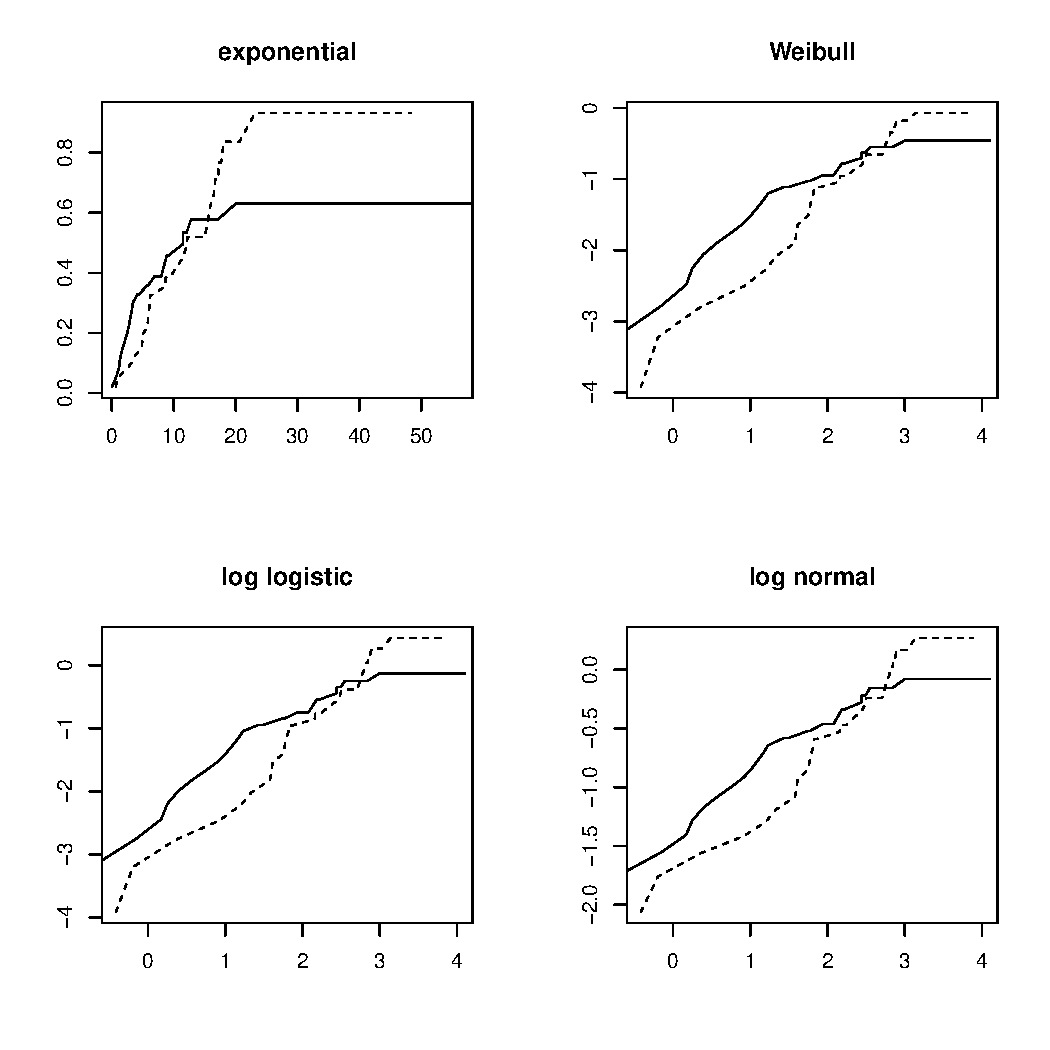
\includegraphics[scale=0.9]{figures/presentation_pic1.pdf}

\caption{Hazard plots for all four parametric models in this section for allo
(solid line) and auto (dashed line) transplant groups. }


\end{figure}

\begin{itemize}
	\item In the first figure the Allo data
appear to be nonlinear while the Auto data is roughly linear.
	\item  For the other three figures, the book claims that they are roughly linear
for both groups.
\end{itemize}

\noindent 
Note that the book generally chops off extreme x values. The probable
justification is the small sample size in the tails although the book
doesn't even mention that it is does this at all, and only a comparison
of the figures that I generated versus figures 12.1-4 in the book
shows that they did in fact do this.

\newpage

\subsection{Checking appropriateness of accelerated failure-time model}
\begin{itemize}
\item When comparing two groups, an alternative to the proportional hazards model is the accelerated failure-time model.
\item A q-q plot can be used to determine the adequacy of this model
\item The plot is based on the fact that, for the accelerated failure-time model,


\begin{align*}
S_{1}(t) & =S_{2}(\theta t),
\end{align*}



where $S_{0}$ and $S_{1}$ are the survival functions in the two
groups and $\theta$ is the acceleration factor.

\item Thus letting $t_{0p}$ and $t_{1p}$ be the $p^{th}$ percentiles
of the groups, we have the following relationship


\begin{align*}
t_{kp} & =S_{k}^{-1}(1-p).
\end{align*}


\item Thus 


\begin{align*}
S_{0}(t_{0p}) & =1-p=S_{1}(t_{1p})=S_{0}(\theta t_{1p}),
\end{align*}



if the model holds.

\item This can be checked by computing the Kaplan-Meier estimators of the
two groups, estimating the percentiles $t_{1p}$, $t_{2p}$ for various
values of $p$, and then plotting the estimated percentiles in group
$1$ against the estimated percentiles in group $2$. If the assumption
holds, the graph should be a straight line with slope $\theta$.\end{itemize}

\noindent{\textbf{Example}  12.1 (continued)}

\noindent Again consider the Allo-Auto data set. A Kaplan-Meier estimate
is calculated for each group and the percentiles $p=.05,.1,\cdots,.35$
are calculated for each group and plotted against each other below
.

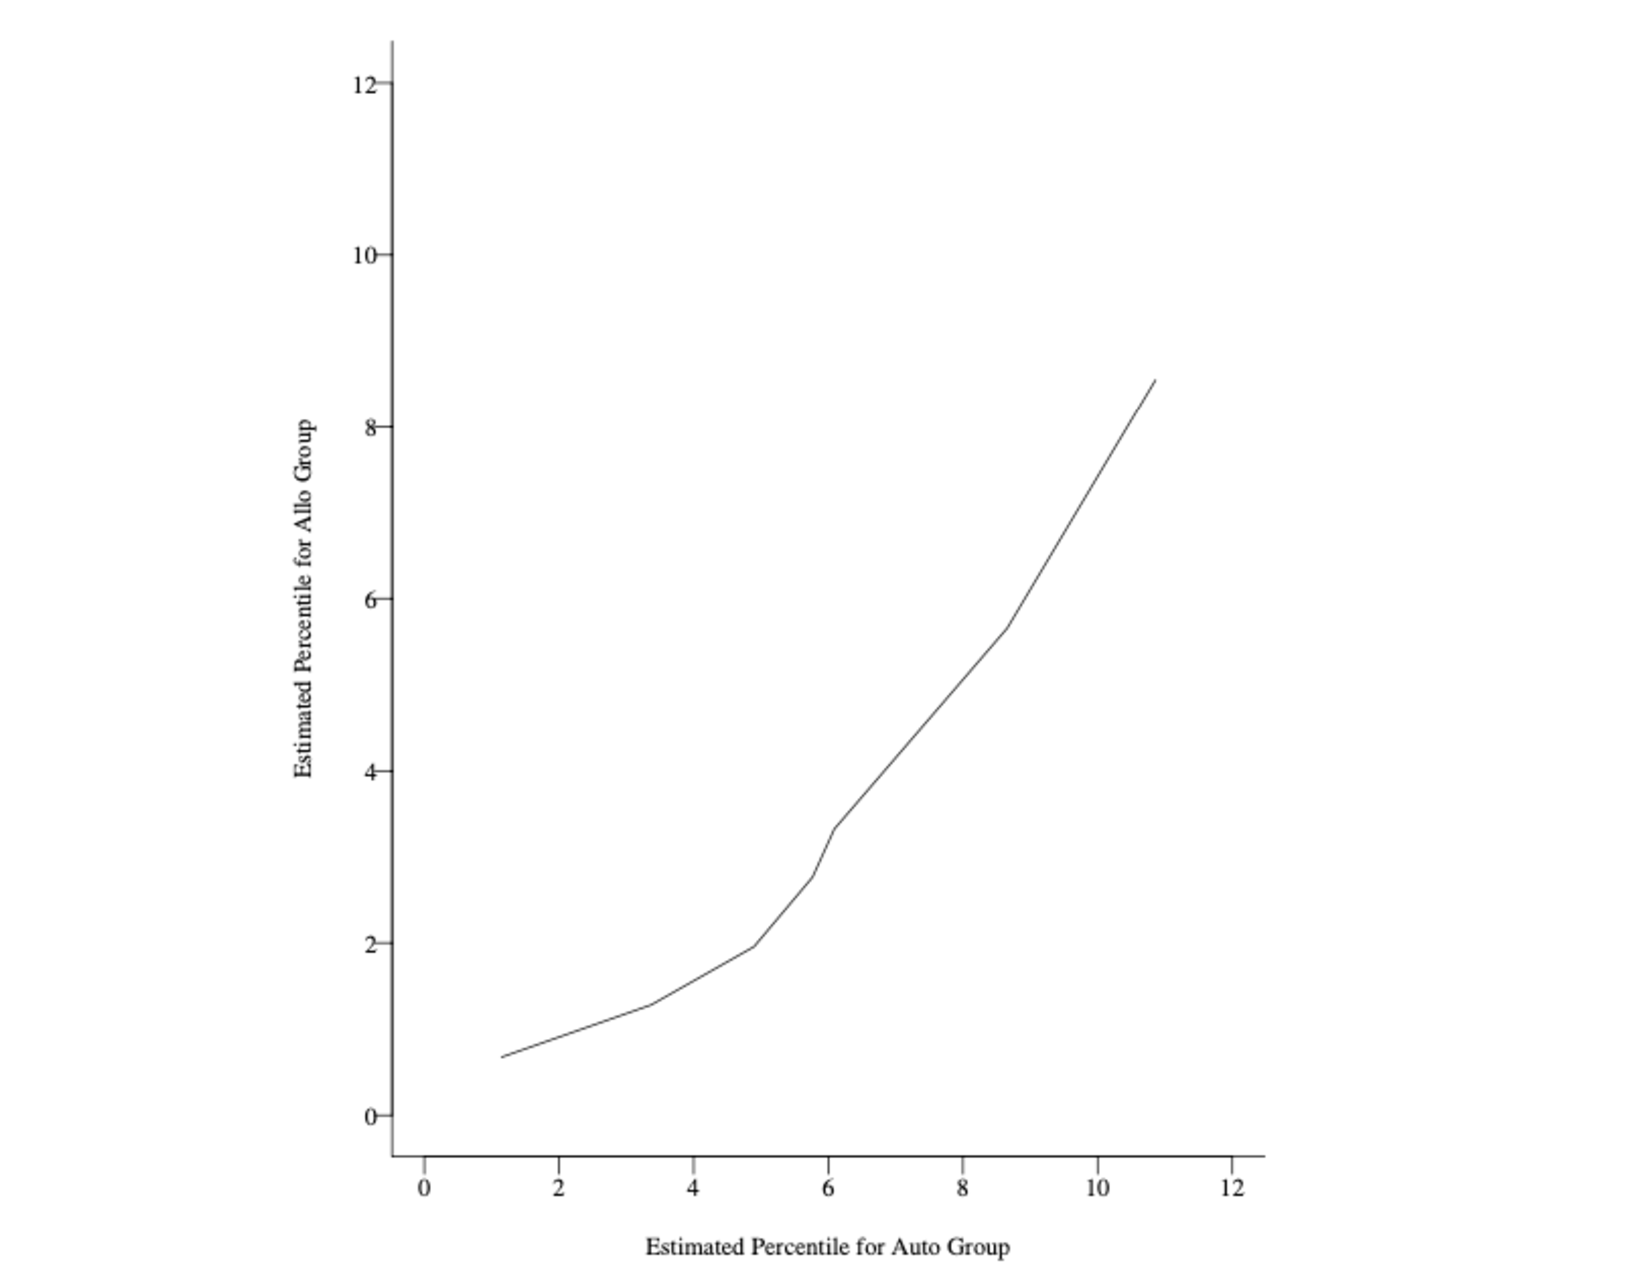
\includegraphics[scale=0.5]{figures/presentation_pic2.pdf}



Note that only a portion of the range $.05$ to $.35$ is actually
plotted above, but the portion that is plotted looks roughly linear.
The figure appears to have a slope of about $\theta=0.6$.


\subsection{Parametric residuals}

For the parametric regression problem, analogs of the residual plots described in Chapter 11 can be made with a redefinition of the various residuals to incorporate the parametric form of the baseline hazard rates.

\subsubsection{Cox-Snell residuals}
\begin{itemize}
\item The Cox–Snell residual is defined as $r_{j}=\widehat{H}(T_{j}|\mathbf{Z}_{j})$, where $\widehat{H}$
is the fitted model. If the model fits the data, then the $r_{j}'s$
should have a standard exponential distribution so that a hazard plot
of $r_{j}$ versus the Nelson-Aalen estimator of the cumulative hazard
of the $r_{j}'s$ should be a straight line with slope 1.
\item The Cox Snell residuals of four parametric models are tabulated below.
\end{itemize}
\begin{center}


\begin{tabular}{|c|c|}
\hline 
\multicolumn{2}{|c}{Cox-Snell residuals}\tabularnewline
\hline 
\hline 
Exponential &
$\widehat{\lambda}t_{i}\exp\left\{ \widehat{\mathbf{\beta}}^{T}\mathbf{Z}_{i}\right\} $\tabularnewline
\hline 
Weibull &
$\widehat{\lambda}\exp\left\{ \mathbf{\widehat{\beta}}^{T}\mathbf{Z}_{i}\right\} t_{1}^{\widehat{\alpha}}$\tabularnewline
\hline 
Log logistic &
$\log\left[\frac{1}{1+\widehat{\lambda}\exp\left\{ \widehat{\mathbf{\beta}}^{T}\mathbf{Z}_{i}\right\} t_{i}^{\widehat{\alpha}}}\right]$\tabularnewline
\hline 
Log normal &
$\log\left[1-\Phi\left(\frac{\log T_{i}-\mathbf{\widehat{\mu}}-\mathbf{\widehat{\gamma}}^{T}\mathbf{Z}_{i}}{\widehat{\sigma}}\right)\right]$\tabularnewline
\hline 
\end{tabular}

\end{center}
\begin{itemize}


\item Equivalently we can analyze the data with the standardized residuals


\begin{align*}
s_{j} & =\frac{\log T_{j}-\widehat{\mu}-\mathbf{\widehat{\gamma}}^{T}\mathbf{Z}_{j}}{\widehat{\sigma}}
\end{align*}


\end{itemize}

\noindent{\textbf{Example} 12.2}

\noindent In Figures 12.6–12.9, the cumulative hazard plots for the Cox–Snell residuals are shown for the exponential, Weibull, log logistic and log normal regression models for the laryngeal cancer data. We see from these plots that all four models give reasonable fits to the data, the best being the log normal and log logistic models.

\begin{figure}[!ht]
  \centering
  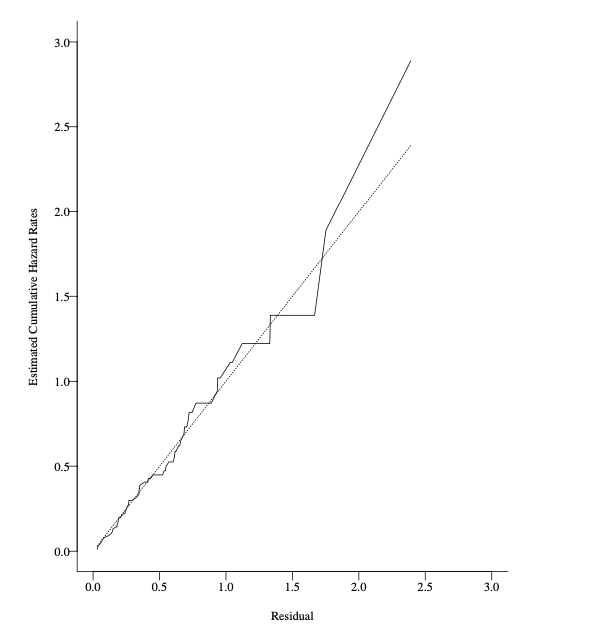
\includegraphics[width=.2\textwidth]{figures/figure1}\quad
  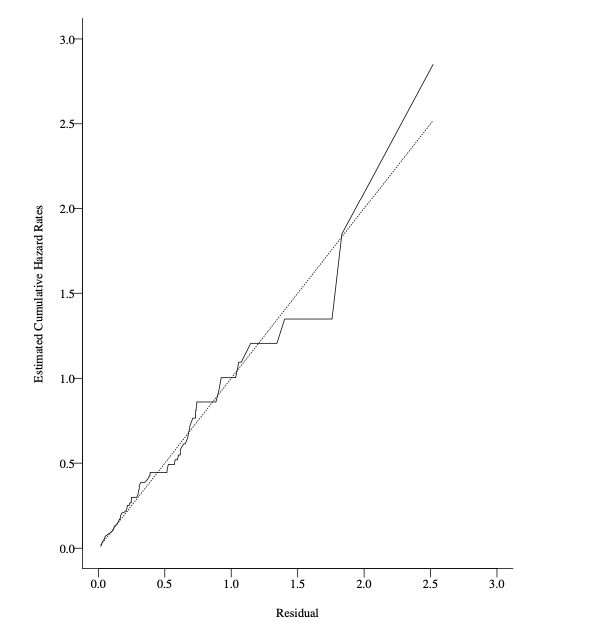
\includegraphics[width=.2\textwidth]{figures/figure2}\\
  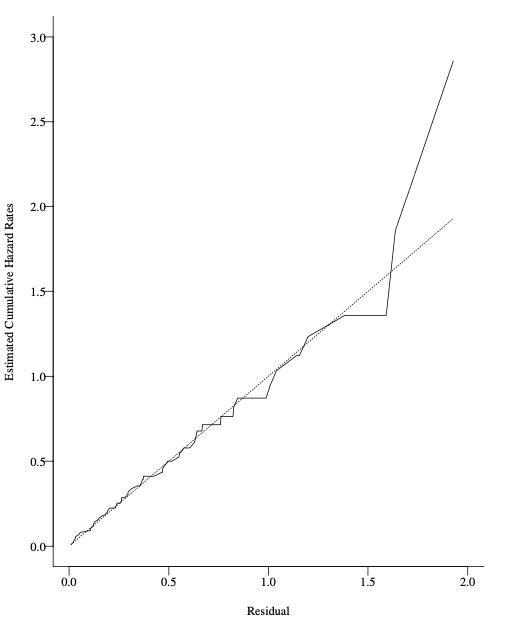
\includegraphics[width=.2\textwidth]{figures/figure3}\quad
  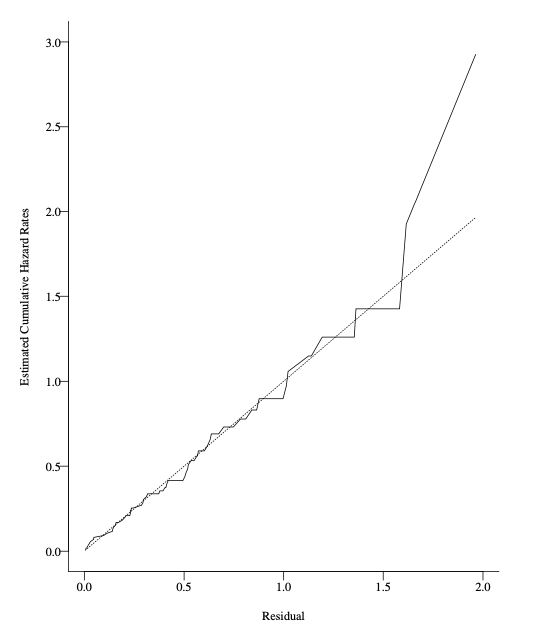
\includegraphics[width=.2\textwidth]{figures/figure4}
  \caption{Cox–Snell residuals to assess the fit of (a) Exponential, (b) Weibull, (c) Log-logistic and (d) Log-normal regression model for the laryngeal cancer data set}
  \label{fig:sub1}
\end{figure}

\newpage 

\subsubsection{Martingale and deviance residuals}
\begin{itemize}
\item The Martingale residual is defined as


\begin{align*}
M_{j} & =\delta_{j}-r_{j}.
\end{align*}


\item The deviance residual is defined as


\begin{align*}
D_{j} & =\mbox{sign}[M_{j}]\left\{ -2\left[M_{j}+\delta_{j}\log(\delta_{j}-M_{j})\right]\right\} ^{1/2}.
\end{align*}


\item As with the Cox model, the Martingale residual is an estimate of the
excess number of deaths seen in the data, but not predicted by the
model.
\item The derivation of the Martingale in the Cox model does not hold here,
but the name is the same because of the similar form
\item The deviance residuals are an attempt to make the Martingale residuals
symmetric about $0$.
\item Plots of either the Martingale or deviance residuals against time,
observation number, or acceleration factor provides a check of model
adequacy
\item Basically, the use of the residuals is the same as in the previous
chapter for the Cox model. Only their derivation has changed.\end{itemize}

\noindent{\textbf{Example} 12.2(Continued...)}
\begin{itemize}
	\item The fit of the log logistic regression model to the laryngeal cancer data using the deviance residuals is examined here.
	\item Below is a plot of the deviance residuals versus time on study.
\end{itemize}
\begin{figure}[h!]
	\centering
  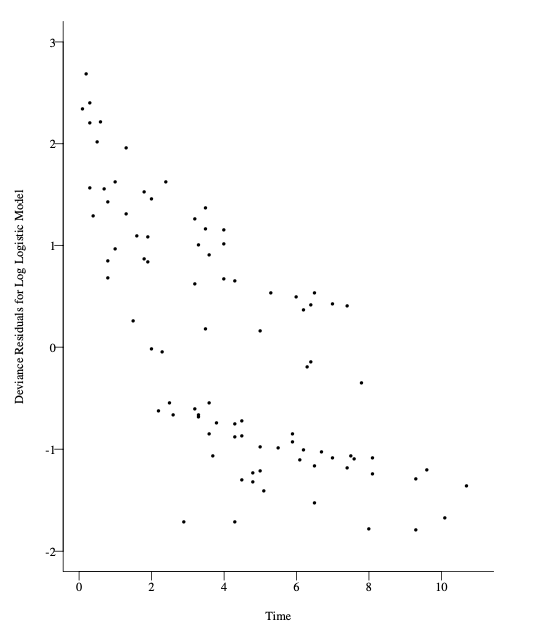
\includegraphics[width=0.5\textwidth]{figures/martingale}
  \caption{Deviance residuals from the log logistic regression model for laryngeal cancer patients}
\end{figure}
\begin{itemize}
	\item Here, we see that the deviance residuals are quite large for small times and that they decrease with time.
	\item This suggests that the model underestimates the chance of dying for small t and overestimates this chance for large t.
	\item However, there are only a few outliers early, which may cause concern about the model. 
\end{itemize}

\subsection{Practical Note}
Martingale and deviance residuals for these parametric models are available in S-Plus.

\end{document}
